%% 
%% Copyright 2007, 2008, 2009 Elsevier Ltd
%% 
%% This file is part of the 'Elsarticle Bundle'.
%% ---------------------------------------------
%% 
%% It may be distributed under the conditions of the LaTeX Project Public
%% License, either version 1.2 of this license or (at your option) any
%% later version.  The latest version of this license is in
%%    http://www.latex-project.org/lppl.txt
%% and version 1.2 or later is part of all distributions of LaTeX
%% version 1999/12/01 or later.
%% 
%% The list of all files belonging to the 'Elsarticle Bundle' is
%% given in the file `manifest.txt'.
%% 

%% Template article for Elsevier's document class `elsarticle'
%% with numbered style bibliographic references
%% SP 2008/03/01

\documentclass[preprint,11pt]{elsarticle}

%% Use the option review to obtain double line spacing
 %\documentclass[authoryear,preprint,review,12pt]{elsarticle}

%% Use the options 1p,twocolumn; 3p; 3p,twocolumn; 5p; or 5p,twocolumn
%% for a journal layout:
%% \documentclass[final,1p,times]{elsarticle}
%% \documentclass[final,1p,times,twocolumn]{elsarticle}
%% \documentclass[final,3p,times]{elsarticle}
%% \documentclass[final,3p,times,twocolumn]{elsarticle}
%% \documentclass[final,5p,times]{elsarticle}
%% \documentclass[final,5p,times,twocolumn]{elsarticle}

%% For including figures, graphicx.sty has been loaded in
%% elsarticle.cls. If you prefer to use the old commands
%% please give \usepackage{epsfig}

%% The amssymb package provides various useful mathematical symbols
\usepackage{amssymb}
%% The amsthm package provides extended theorem environments
%% \usepackage{amsthm}

%% The lineno packages adds line numbers. Start line numbering with
%% \begin{linenumbers}, end it with \end{linenumbers}. Or switch it on
%% for the whole article with \linenumbers.
%% \usepackage{lineno}

\usepackage{graphicx}
\graphicspath{ {images/}}
%\usepackage[boxed]{algorithm2e}
%\usepackage{algpseudocode}
\usepackage{slashbox}
\journal{Decision Support Systems}

\begin{document}

\begin{frontmatter}

%% Title, authors and addresses

%% use the tnoteref command within \title for footnotes;
%% use the tnotetext command for theassociated footnote;
%% use the fnref command within \author or \address for footnotes;
%% use the fntext command for theassociated footnote;
%% use the corref command within \author for corresponding author footnotes;
%% use the cortext command for theassociated footnote;
%% use the ead command for the email address,
%% and the form \ead[url] for the home page:
%% \title{Title\tnoteref{label1}}
%% \tnotetext[label1]{}
%% \author{Name\corref{cor1}\fnref{label2}}
%% \ead{email address}
%% \ead[url]{home page}
%% \fntext[label2]{}
%% \cortext[cor1]{}
%% \address{Address\fnref{label3}}
%% \fntext[label3]{}

\title{Evaluation of spell correction on noisy OCR data}

%% use optional labels to link authors explicitly to addresses:
%% \author[label1,label2]{}
%% \address[label1]{}
%% \address[label2]{}

\author{Aayushee Gupta, Haimonti Dutta}

\address{}



\begin{abstract}
%% Text of abstract
Optical Character Recognition (OCR) of historical text often leads to several kinds of spelling errors. Existing spell correction algorithms do not present a rigorous performance evaluation of the spell correction process. In this paper, we present a novel N-gram based algorithm for checking the accuracy of spell correction which can handle noisy and cleaned text of different lengths.
 %First, an edit distance based spell correction algorithm is presented which forms the basis of the evaluation mechanism. The goal of the Spell Correction Evaluation (SCE) algorithm is to measure accuracy of the text corrected by the spell correction algorithm against manually corrected data. N word grams are used to make word-to-word correspondences between the corrected text and the noisy OCR text - each token is then annotated as a True/False Positive/Negative of the correction process. 
The algorithm relies on appropriately choosing a window of N-words and aligning them in three parallel corpora - noisy OCR, corrected, and cleaned and annotated text (ground truth). Empirical results of spell correction on 300 news articles from the ``The Sun" newspaper, Nov- Dec 1894 are presented on edit distance and context sensitive based spell correctors. The Spell Correction Evaluation (SCE) algorithm evaluates their AUC values to be 0.49 and 0.56 respectively. We posit that this novel algorithm for spell correction evaluation has a wide applicability and can play a crucial role in analyzing large volumes of digitized OCR text.

\end{abstract}

\begin{keyword}
%% keywords here, in the form: keyword \sep keyword
 OCR \sep Spell Correction \sep Spell Correction Evaluation \sep Historical Newspaper Archives
%% PACS codes here, in the form: \PACS code \sep code

%% MSC codes here, in the form: \MSC code \sep code
%% or \MSC[2008] code \sep code (2000 is the default)

\end{keyword}

\end{frontmatter}

%% \linenumbers

%% main text


\section{Introduction}

OCR of typed, handwritten or printed text is widely used to obtain digitized text which can be edited, searched, stored and displayed efficiently(\cite{torget2011mapping,palfray2012logical}). It is used in various applications such as banking, digital libraries \cite{mcmurdo2013vermont} and repositories, number plate recognition, and handwriting recognition \cite{singh2012survey}. However, the OCR scanning of printed text generates a lot of garbled text which renders them inadequate for any such tasks. Refinement of such noisy OCR text through spell correction can make them useful for text mining tasks (\cite{dutta2011learning}, \cite{yang2011topic}).

Most spell correction algorithms have focused on improving the correction model and either do not give a detailed performance evaluation of the algorithm post spell correction or the evaluation measures used are not able to completely analyze the performance of such algorithms.  
A major problem that surfaces when evaluating a spell corrector is that the text has to be verified against the original text (ground truth) to estimate its performance. This one-to-one verification may lead to word alignment problems, since the corrected and original text can be of different lengths.
In this paper, we describe the development of an N-word grams Spell Correction Evaluation (SCE) algorithm that can automatically evaluate a spell correction algorithm by using an N-word window to align three parallel corpora - the noisy OCR, corrected and original/ manually cleaned text. 
We present the performance evaluation results of applying our SCE algorithm on two  commonly used spell correction techniques - Edit distance and Context Sensitive spelliing correction on 300 OCR historical newspaper articles of ``The Sun" newspaper published in Nov-Dec 1894. 

\noindent \textbf{Organization: } This paper is organized as follows: related work is described in Section~\ref{spell:rw}; characteristics of the OCR data and its annotation in Section~\ref{spell:errors}; spelling correction and evaluation algorithms in Section~\ref{spell:algo}; empirical evaluation in Section~\ref{spell:results} followed by discussion and future work in Section~\ref{spell:fw}. 

\section{Related Work}
\label{spell:rw}

Spelling correction algorithms have been vastly discussed in literature but either their evaluation measures and data analysis are not accurate or they do not take all types of OCR errors into consideration.
Kukich\cite{kukich1992techniques} comprehensively discusses various spelling correction techniques based on non word, isolated word and real word spelling errors. N-gram analysis, dictionary lookup and probabilistic techniques (\cite{strohmaier2003lexical}, \cite{ringlstetter2007text}) are used for correcting isolated and nonword errors while context-dependent techniques are used mostly for correcting real word errors including the correction of word split and join errors \cite{elmi1998spelling}.
N-gram techniques work by examining each n-gram in the text string and comparing against a pre-compiled table of n-gram statistics to retrieve the correct word while dictionary look up techniques directly check whether the text string appears in the dictionary using string matching algorithms. Both techniques require a dictionary or a large text corpus and take frequency of n-grams or word occurrence into account in order to find the correct spelling .
Probabilistic techniques use transition and word confusion probabilities to estimate likelihood of the correction in order to rank and retrieve correct word spelling.
On the other hand, Context-dependent techniques require contextual information and use either extensive NLP techniques or Statistical Language Modeling (SLM) for spelling correction.
Bassil and Alwani\cite{bassil2012ocr} use Google 1-5 gram word dataset to gain context information in order to determine the correct words sequence in the text for correction.
Tong and Evans\cite{tong1996statistical} use Statistical Language Modeling (SLM) approach involving information from letter n-grams, character confusion and word bi-gram probabilities to perform context sensitive spelling correction obtaining a 60 percent error reduction rate. All these spelling correction techniques have developed over time and have been used in combination to achieve improved accuracy \cite{brill2000improved}. Agarwal et al.\cite{agarwal2013utilizing} use a combination of Google suggestions, LCS and character confusion probabilities for choosing the correct spelling on a small set of historical newspaper data and achieve recall and precision of $51\%$ and $100\%$ respectively.

The edit distance approach, suggested initially by Wagner and Fischer\cite{wagner1974string}, is a dictionary lookup approach commonly used for OCR data correction because of the large number of substitution errors in OCR data  \cite{kukich1992techniques}\cite{christen2006comparison} which can be corrected using this technique. String edit distance approaches with faster correction are discussed in \cite{marzal1993computation},\cite{schulz2002fast}  with variants like Levenshtein automata and normalized edit distance.
% WHERE DO I PUT THIS? ? ? Holley et al.\cite{holley2009good} posit that it is difficult to measure the true and improved accuracy of OCR and recording character confidence is not equivalent to the accuracy of the OCR text.
%There has not been enough research work regarding automatic evaluation of word-by-word post spelling correction on OCR dataset consisting of Word Split and Join errors. 
All of the above algorithms are evaluated based on the percentage of spelling errors corrected or reduction in the word error rate and do not consider the word alignment problem arising due to word split and join errors in the OCR text. 

Semi-automatic spelling correction systems \cite{taghva2001ocrspell} require user interaction in order to perform complete correction and system evaluation. Rice\cite{rice1996measuring} discusses OCR errors similar to the ones in our dataset. Their algorithm evaluates edit distance spelling correction by estimating word accuracy; the length of LCS between correct and incorrect strings on a page-by-page level is used as the relevant metric. 
The evaluation strategy works correctly but the definition of accuracy does not give a complete coverage of the spell correction as it does not provide any information on the errors missed by the spelling corrector due to lack of word by word comparison/alignment during the evaluation procedure.

---ADD RELATED WORK REGARDING LINGPIPE BASED CONTEXT SENSITIVE SPELL CORRECTION HERE. 

---ADD RELATED WORK REGARDING RECENT PAPERS READ ON SPELLING CORRECTION EVALUATION. (REYNAERT PAPERS, Compound words paper)

--specifically mention that most of the evaluation mechanisms use OCR and true word pairs for measuring the algorithm performance which is not suitable for a complete evaluation of the spelling correction algorithm where the dataset has word split and join errors.



\section{Data}
\label{spell:errors}
\begin{figure}[hbt]
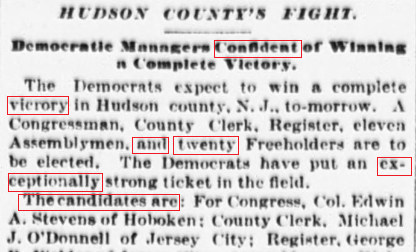
\includegraphics[scale=0.75]{originalimage}
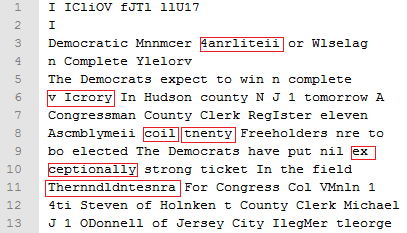
\includegraphics[scale=0.80]{ocr}
\caption{Scanned Image of a Newspaper article (left) and its OCR raw text (right)}
\label{figure:1}
\end{figure}

%\noindent An individual OCR text article has at least one or more of the following types of spelling errors: (1) \textbf{Real word errors: }include words that are spelled correctly in the OCR text but still incorrect when compared to the original newspaper article image. %Example\footnote{All the examples are illustrated in Figure~\ref{figure:1}}: ``coil"  has been correctly spelled in the OCR text  but should have been ``and" according to the original newspaper article. (2) \textbf{Non-real word errors: }include words that have been misspelled %due to some insertion, deletion, substitution or transposition of characters from a word. Example: ``tnenty" in the OCR text has a substitution error (`n' should have been `w') which is actually ``twenty" according to the original newspaper article. (3) \textbf{Non-word errors: %}include words that have been spelled incorrectly and are a combination of alphabets and numerical characters. Example:  ``4anrliteii" which is a combination of alphabets and number and should have been ``confident" as per the original newspaper article. (4) \textbf{New %Line errors: }include words that are separated by hyphens where part of a word is written on one text line and remaining part in the next line. Example: ``ex-ceptionally" where ``ex" occurs on one line while ``ceptionally" in the next and due to no punctuation in the text, %they are treated as separate words in OCR text. (5) \textbf{Word Split and Join errors: }include words that either get split into one of more parts or some words in a sentence get joined to a make a single word. Example: ``Thernndldntesnra" in the OCR text is actually a %combination of three words ``The candidates are" while the words ``v Icrory" are actually equivalent to a single word ``victory" when compared with the original news article.



 An individual OCR text article has at least one or more of the following types of spelling errors:
\begin{description}
 \item[$\bullet$Real word errors] include words that are spelled correctly in the OCR text but still incorrect when compared to the original newspaper article image. For example: In Figure~\ref{figure:1}, the word ``coil"  has been correctly spelled in the OCR text  but should have been ``and" according to the original newspaper article. 
 \item[$\bullet$Non-real word errors] include words that have been misspelled due to some insertion, deletion, substitution or transposition of characters from a word. For eg. In Figure~\ref{figure:1}, the word ``tnenty" in the OCR text has a substitution error (`n' should have been `w') which is actually ``twenty" according to the original newspaper article.
 \item[$\bullet$Non-word errors] include words that have been spelled incorrectly and are a combination of alphabets and numerical characters. For example: In Figure~\ref{figure:1}, the word ``4anrliteii" which is a combination of alphabets and number and should have been ``confident" as per the original newspaper article.
\item[$\bullet$New Line errors] include words that are separated by hyphens where part of a word is written on one text line and remaining part in the next line. For example: In Figure~\ref{figure:1}, the word ``ex-ceptionally" where ``ex" occurs on one line while ``ceptionally" in the next and due to no punctuation in the text, they are treated as separate words in OCR text.
\item[$\bullet$Word Split and Join errors] include words that either get split into one of more parts or some words in a sentence get joined to a make a single word. For example: In Figure~\ref{figure:1}, the word ``Thernndldntesnra" in the OCR text is actually a combination of three words ``The candidates are" while the words ``v Icrory" are actually equivalent to a single word ``victory" when compared with the original news article.
\end{description} 

\subsection{Data Statistics}


\subsection{Manual Annotation of Data}
In order to obtain the original cleaned text from the OCR data, we used manual annotators who annotated the OCR articles from their newspaper images.
--DESCRIBE THE ANNOTATION EXPERIMENT HERE.




\section{Theory}
\label{spell:algo}
%Several kinds of spelling errors can exist in the OCR text as described in the previous section. 
%
%
%% DOUBT: Do the following lines need to be removed?
%%The garbled OCR dataset  needs to be refined by correcting the text with the help of a human editor manually or automatic spelling corrector. Due to the huge size of dataset, human editing would be extremely time consuming and expensive making it impossible and indicating requirement of a spelling correction technique. 
%We use edit distance algorithm for spelling correction because of its speed and ability to correct OCR errors compared to the n-gram approach \cite{chattopadhyaya2013fast}. Context-dependent spelling correction is not used because of unavailability of n-gram words corpus or ground truth dataset containing OCR and true word pairs.
%

\subsection{ Edit Distance Spelling Corrector}
\label{spell:algorithm}
The Edit Distance algorithm based on Levenshtein distance\cite{levenshtein1966binary} has been used for spelling correction. It is an isolated word correction technique that uses dictionary based-look up and the distance between strings for matching the text and correcting it. An ``edit distance"\footnote{Our edit distance algorithm corrects non-real word spelling errors by making at most 2 operations of insertion, deletion and substitution of letters in the word. The choice of 2 is governed by the trade off between algorithm runtime and quality of spelling correction. The spelling corrector has been designed as suggested by Peter Norvig\texttt{ http://norvig.com/spell-correct.html}.} corresponds to the minimum number of insertions, deletions, and substitutions required to transform one string into another. %The algorithm requires a dictionary which is used to check if each word of the text exists in it or not. If it does, then no change is made to the word; otherwise, a candidate list of words is created from the word to be corrected by inserting, substituting or deleting up to 2 letters from it.  This list of words is returned as suggestions for the word to be corrected. The correction is made with the word formed from lowest edit distance and occurring with more frequency in the dictionary. This makes the edit distance algorithm dependent on the type of dictionary chosen for correction.
% which means the dictionary must be well chosen for spelling correction of a specific document collection. 
%The algorithm is made to run fast by reading the dictionary only once and keeping a data structure in memory for its word counts which can be referred to whenever a word comes up for correction.


\subsection{Context Sensitive Spelling Corrector}



\subsection{Spelling Correction Algorithm Evaluation }
\label{spell:sce}
For evaluating the performance of spell correction, the raw OCR text and OCR text after application of spelling correction algorithm (corrected text) needs to be compared with the original newspaper text. The OCR text is extremely garbled with Word Split and Join errors due to which word-to-word alignment with the original newspaper text is impossible,i.e., the raw OCR and original newspaper text are of different lengths. A novel algorithm,Spelling Correction Evaluation (SCE) based on N-gram approach is proposed for automatic evaluation of the corrected text. %word-by-word against the manually corrected subset of the news articles dataset. 
The SCE algorithm can be used for evaluation of any type of spelling correction algorithm - dictionary look up, context sensitive or probabilistic spell correction algorithms.
The  following metrics are used for estimating the performance:
%\noindent \textbf{Evaluation Parameters}
%\begin{description}
% \item[$\bullet$Accuracy]
(1) \textbf{Accuracy }This requires calculation of the number of OCR errors that got corrected when compared to the original newspaper text. Specifically,
%The measure has been chosen so as to include the complete text coverage and not just check for words that get corrected after spell correction as in the latter case, the  number of False Postivies and True Negatives get missed which does not give the correct measure of how well the spell corrector works. The formula used for calculating Accuracy is defined by Manning and Schutze,1999 (p.268-269) as follows:
$Accuracy=  \frac{TP+TN} {TP+ FP + TN + FN}$ where, $TP$=Number of True Positives, $TN$=Number of True Negatives, $FP$=Number of False Positives, $FN$=Number of False Negatives. %The aim of the SCE algorithm is to make a word-to-word correspondence between the OCR corrected text and the original newspaper text and to mark each token in the OCR text as a $TP$, $FP$, $TN$ or $FN$. 
Reynaert and Martin\cite{reynaert2008all} suggest a way to define these terms by distinguishing between correct words and incorrect words in the text through the set of non-target, target and selected words and use Precision and Recall evaluation measures for measuring performance of spelling correction which we adapt for this work. %According to our SCE algorithm, a ``true positive" is said to occur when a word from the OCR text gets corrected and the corrected spelling matches the one in original article text while a ``false positive" occurs if the corrected spelling does not match the corresponding word in the original article text. A ``true negative" occurs when a word does not get corrected by the algorithm as it is already correct and matches the correct word in the original text also. On the other hand, a ``false negative" occurs when the algorithm is unable to correct the word (there is no change in spelling of the word) and it does not match the corresponding word in the original text but should have been corrected.
(2) \textbf{Time taken for Spelling Correction } The time for correcting the text is also noted for benchmarking correction of large datasets.

%\end{description}

\noindent \textbf{N-Word Grams Spelling Correction Evaluation(SCE) Algorithm}
To make the correspondence between corrected and original OCR text, a window of N-word grams in the original newspaper text is considered which can be seen in a diagrammatic representation in Figure~\ref{figure:2}.
\begin{figure} [!htb]
\centering
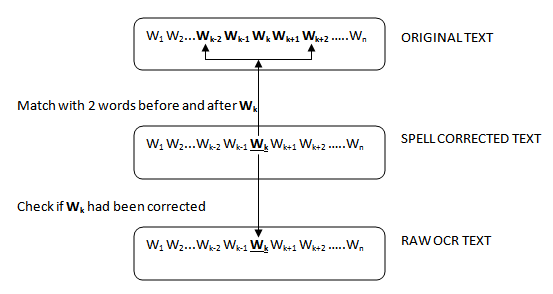
\includegraphics[scale=0.8]{ngram}
\caption{Schematic diagram for alignment of spell corrected article text with original article text for a word $W_{k}$}
\label{figure:2}
\end{figure}
\noindent For each token in the spell corrected text, the corresponding token in the original text article along with 2 tokens before and 2 tokens after it are considered for alignment\footnote{ The choice of N=2 is based on the Word Split and Join errors in the dataset. This value can be set appropriately by considering the maximum difference of lengths in each line of OCR and original text in the dataset.}.
If the token being considered matches with any word in the original text article word's window and its spelling has been corrected when compared to the corresponding token in raw OCR text, then it is marked as a ``True Positive" which is actually rewarding the Spell corrector for making the correct spelling change. A ``False Positive" is marked if it does not match any of the words despite its spelling being corrected. 
%If the token being considered matches any of the words in the words window but no spelling correction has been made for it, then it is marked as a ``True Negative" and if it does not match any word in the window and the spelling corrector also did not correct it, then it is marked as a ``False Negative" as the word got missed by the corrector. 
%Several cases could occur during alignment like difference in the lengths of line text between OCR and Original text or while considering the first, second or the last tokens from the Corrected line text for which the corresponding word window in Original text needs to be smaller. All such cases have been covered in SCE Algorithm 1 which calls function `MatchWordGrams' (Algorithm2) for these different cases. 
%%%%DOUBT---USE THIS TABLE INSTEAD OF ALGORITHMS 1 AND 2???
Table~\ref{table1} describes the the process of marking each token in the corrected text as a TP, TN, FP or FN in each text article for calculation of accuracy. The final values of TP, TN, FP and FN are accumulated throughout the dataset to calculate accuracy.
 
\begin{table}[ h]
\centering
\caption{Calculation of accuracy in SCE algorithm}
\label{table1}
\begin{tabular}{|l|l|l|l|l|}
\hline
\backslashbox{Criteria to be checked}{Evaluation Metric}          & TP  & TN  & FP  & FN \\ \hline
Match found in N-word window? & Yes & Yes & No  & No \\ \hline
Spell correction was done?  & Yes & No  & Yes & No \\ \hline
\end{tabular}
\end{table}

\noindent Several scenarios could arise during the word alignment process due to difference in the lengths of text between OCR and original text. All such cases are depicted in Table~\ref{table2} which describes the window size of tokens to match in the original text (from j=starting index to ending index) for every token \textit{i} of the corrected text.

\begin{table}[h]
\centering
\caption{Different cases for word alignment}
\label{table2}
\scalebox{0.9}{
\begin{tabular}{|l|l|l|}
\hline
\backslashbox{Token index of CorrectedLine(i)}{Token index of OriginalLine}                                                   & Starting index (j)         & Ending index (j)         \\ \hline
Length{[}CorrectedLine{]} \textless4 or Length{[}OriginalLine{]}\textless4                                 & 0                          & Length{[}OriginalLine{]} \\ \hline
i=0                                                                                                        & 0                          & 3                        \\ \hline
i=1                                                                                                        & 0                          & 4                        \\ \hline
i=Length{[}CorrectedLine]-2 	&i-2			&Length{[}OriginalLine{]} \\ \hline
i=Length{[}CorrectedLine{]}-1	 & i-2                        & Length{[}OriginalLine{]} \\ \hline
i=Length{[}CorrectedLine{]}	 & i-2                        & Length{[}OriginalLine{]} \\ \hline
i=Length{[}CorrectedLine+1{]} & i-2                        & Length{[}OriginalLine{]} \\ \hline
i\textgreater=Length{[}CorrectedLine{]}+2                                                                  & Length{[}OriginalLine{]}-3 & Length{[}OriginalLine{]} \\ \hline
Any other value of i                                                                                            & i-2                        & i+3                      \\ \hline
\end{tabular}}
\end{table}

\noindent A limitation of the SCE algorithm is that it requires all 3 versions of a newspaper article (Original, Corrected and OCR) to have the same number of lines as alignment of line texts is performed. In case of difference in the number of lines of text due to some Word Split and Join errors, the word's window needs to be extended so as to cover previous and next line texts also for alignment.


%\begin{algorithm}[!h]
%\caption{SCE Algorithm for Spell Correction}
%  \KwIn{Ocr.txt,Corrected.txt,Original.txt}
%  \KwOut{Spell Corrector Accuracy }
%\SetKwFunction{MatchWordGrams}{MatchWordGrams}%
% $OcrLine$:=a line of text from Ocr.txt\;
% $CorrectedLine$:=a line of text from Corrected.txt\;
% $OriginalLine$:=a line of text from Original.txt\;
% $tp \leftarrow $0  $fp \leftarrow $0 $tn \leftarrow $0 $fn\leftarrow $0\;  
%	\For{(int i=0; i $<$ CorrectedLine.length ; i++) }
%	{
%
%    \If{(CorrectedLine.length$<$4 $||$ OriginalLine.length$<$4)}
%	{		
%    	\MatchWordGrams{(OcrLine,CorrectedLine,OriginalLine,0,OriginalLine.length,i)}\; 
%	}
%    \Else{
%   \If {(i==0)}
%   {
%\MatchWordGrams{(OcrLine,CorrectedLine,OriginalLine,0,3,0)}\;
%   }
%   \ElseIf{ (i==1)}
%   {
%\MatchWordGrams{(OcrLine,CorrectedLine,OriginalLine,0,4,1)}\;
%   }
%	\ElseIf{(i==(CorrectedLine.length-2) $||$ (CorrectedLine.length-1) $||$ (CorrectedLine.length) $||$ (CorrectedLine.length+1))}
%	{
%\MatchWordGrams{(OcrLine,CorrectedLine,OriginalLine,i-2,OriginalLine.length,i)}\;
%	}  
%	\ElseIf{(i $>$= CorrectedLine.length+2)}
%	{	
%\MatchWordGrams{(OcrLine,CorrectedLine,OriginalLine,OriginalLine.length-3,OriginalLine.length,i)}\;	
%	}
%	\Else
%	 {
%\MatchWordGrams{(OcrLine,CorrectedLine,OriginalLine,i-2,i+2,i)}\;	
%	}	
%   }
% }
% 	 $Accuracy=(tp+tn)/(tp+tn+fp+fn);$\
%\end{algorithm}
%
%
%
%
%\begin{algorithm}[H]
%\caption{MatchWordGrams Function called by Algorithm 1}
%\begin{algorithmic}
%\Function {MatchWordGrams}{OcrLine, CorrectedLine, OriginalLine, jstart, jend, i}
%  
% \For{(int j=jstart; j$<$jend; j++)}
%  {
%    \If{ ((CorrectedLine[i].equals(OriginalLine[j]))\&\&(!(OcrLine[i].equals(CorrectedLine[i]))))}
%     {
%	  $tp=tp+1$\;
%	  flag0=false\;
%	 \Return $tp$\;
%	  }
%	\ElseIf{((CorrectedLine[i].equals(OriginalLine[j]))\&\&(OcrLine[i].equals(CorrectedLine[i])))}
%	      {
%		 $tn=tn+1$\;
%		  flag1=false\;
%		\Return $tn$\;
%	      }
%}
%
%	 \If{(!(OcrLine[i].equals(CorrectedLine[i]))\&\&flag0==true)}
%	 {
%		    $fp=fp+1$\;
%		   \Return $fp$\;
%            }
%	 
%	 \ElseIf{((OcrLine[i].equals(CorrectedLine[i])) \&\& flag1==true)}
%	 {
%		    $fn=fn+1$\;
%		   \Return $fn$\;
%	 }
%\EndFunction
%\end{algorithmic}
%\end{algorithm}





\textbf{An Illustrative Example } The execution of the SCE algorithm can be demonstrated with the help of the following example:
Consider 3 versions of a scanned image of a newspaper article -- the original text of the scanned image, the raw OCR text and the text after spell correction. %in Figure~\ref{figure:4}. 
Assume, the texts are:

OcrLine= \textit{by tltn rejmrt of th cepert aocountauts who}

CorrectedLine= \textit{by than report of the expert accountants who}

OriginalLine= \textit{by the report of the expert accountants who} 

\noindent Here, for each token of CorrectedLine, we find its index and call the MatchWordGrams function accordingly. For the first token `by' at index i=0 in CorrectedLine, we consider the word window to be ``by the report" (index j=0 to 2) in OriginalLine by matching iteratively with each token to see if there is a match and also if there has been a spelling correction by comparing with the corresponding token in OcrLine. Here, no change was made to the spelling of `by' and it matches with a word in words window, so it is marked as a FN. For the second token `than' at index i=1, we consider the word window to be ``by the report of" (index j=0 to 3) for which there is no match in the window but there has been a spelling correction from `tltn' to `than', which implies the correction was wrong and the token is marked as a $FP$. For the third token `report' at index i=2, we consider the window as ``by the report of the" (index j=0 to 4) in Original Line and find that there is a match in the word window and there has been a spelling correction too from `rejmrt' to `report' which makes this token a $TP$. Similarly, rest of the tokens get marked for each line in the Corrected.txt. 

Another example can be considered from Line 10 in Figure~\ref{figure:3} and Figure~\ref{figure:4} where the number of tokens is different in CorrectedLine and OriginalLine. In such a case, direct alignment between tokens is not possible because of which the words window becomes useful. Here, when the last token `Richmond' of CorrectedLine is considered at index i=3, the corresponding words window becomes ``Jury now sitting at Richmond" (index j=1 to 5) for which there is a match in the words windows and corresponding spelling has also been changed from `tilchmond' to `Richmond' which makes it a $TP$. Had the word window not been considered, the corresponding token at index j=3 in OriginalLine would have been chosen as `sitting' which would have resulted in a $FP$. 
   

\begin{figure}[!htb]
\begin{center}
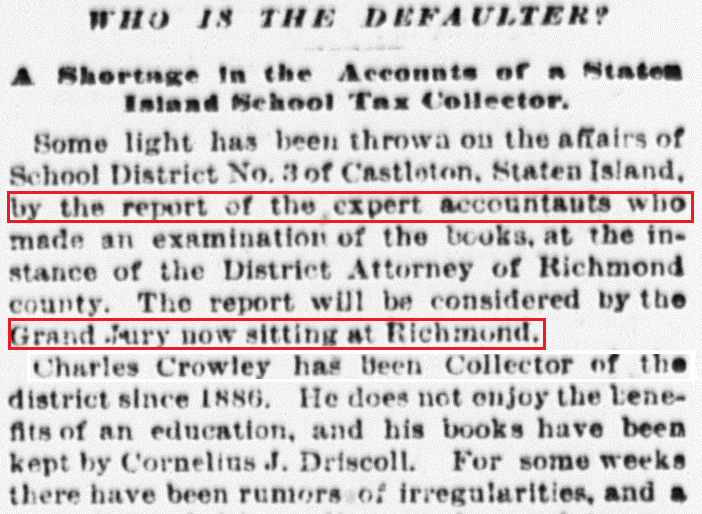
\includegraphics[scale=0.4]{img3}
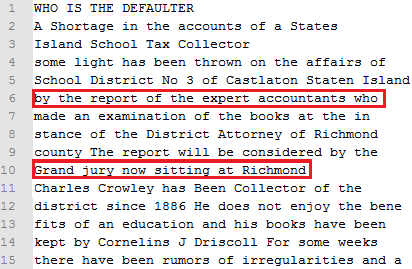
\includegraphics[scale=0.75]{originalimg3}
\caption{Scanned image of a newspaper article (left) along with its original text (right)}
\label{figure:3}
\end{center}
\end{figure}


\begin{figure}[!htb]
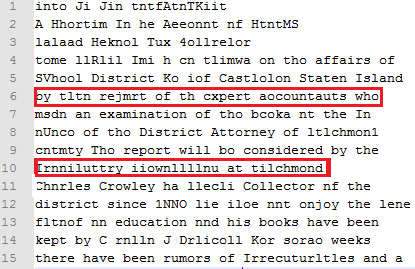
\includegraphics[scale=0.75]{ocr3}
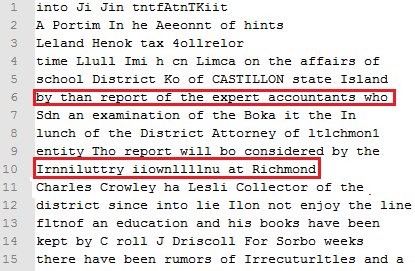
\includegraphics[scale=0.75]{corrected3}
\caption{OCR raw text (left) and Spell corrected text (right) of the article}
\label{figure:4}
\end{figure} 

\section{Empirical Evaluation and Results}
\label{spell:results}

\noindent \textbf{Data Source} 
%%%%DELETE THIS SECTION IF REQUIRED AND MERGE IT WITH THE NEXT SECTION...
The dataset used for empirical evaluation of the algorithm has been obtained from the Chronicling America\footnote{\texttt{http://chroniclingamerica.loc.gov/}} website. It contains scanned newspaper pages published in New York between1890 to 1920. OCR software is run over high
resolution images to create searchable full text of the newspaper articles.

In order to make a newspaper available for searching on the Internet,
the following processes used in \cite{dutta2011learning} must take place: (1) the microfilm copy or
paper original is scanned; (2) master and Web image files are
generated; (3) metadata is assigned for each page to improve the
search capability of the newspaper; (4) OCR software is run over high
resolution images to create searchable full text and (5) OCR text,
images, and metadata are imported into a digital library software
program. 
The scanned newspaper holdings of the NYPL offers a wealth of
data and opinion for researchers and historians.The newspaper titles and digitized pages available through the
Chronicling America website can be searched using the OpenSearch
protocol\footnote{\texttt{http://www.opensearch.org/Home}}.
Unfortunately, the current search facilities are rudimentary and
irrelevant documents are often more highly ranked than relevant ones.
The newspapers are scanned on a page-by-page basis and article level
segmentation is poor or non-existent; the OCR scanning process is far
from perfect and the documents generated from it contains a large
amount of garbled text. In a bid to serve its patrons better, the New
York Public Library employed human annotators to clean headlines of
articles and text, but the process of manually reading all the old
newspapers article-by-article and cleaning them soon became very
expensive. 

\noindent \textbf{Data Statistics }%The OCR text available is on a page-by-page level and no article level segmentation is provided. OCR text dataset is therefore, taken from a PostgreSQL database where article level segmentation of page-level OCR text from Chronicling America is available for
Two months of articles of ``The Sun" newspaper from November-December 1894 consisting of 14020 news articles with a total of 8,403,844 tokens are used for empirical evaluation. %The newspaper database ER diagram \footnote{https://power.ldeo.columbia.edu/twiki/pub/Incubator/BodhiDBDesign/Final ERD.pdf }
%is used to extract the required articles text from the database by dumping complete dataset and extracting individual articles linetext based on their unique ID. 
The text does not have any punctuation and contains a large amount of garbled text containing OCR errors mentioned in Section~\ref{spell:errors}.

\noindent \textbf{Experimental Procedure and Results}

\noindent \textbf{Aim: }The aim of our experiments is to answer the following question:
How good is the spell corrector? The metrics for evaluation are accuracy and time taken to correct the text.


\noindent \textbf{Materials: }The spelling correction algorithm is used to correct all the 14020 OCR raw text articles in the dataset. The dictionary used for look-up is a concatenation of several public domain books from Project Gutenberg and lists of most frequent words from Wiktionary and the British National Corpus\footnote{http://norvig.com/big.txt}. This is augmented with a large people names list which is obtained  by running Stanford NER-CRF parser on subsets of the ClueWeb12 dataset made available in the TREC 2013 Crowdsourcing Track\footnote{http://boston.lti.cs.cmu.edu/clueweb12/TRECcrowdsourcing2013/}. This enhanced dictionary has been used to give special consideration to correction of person names in the dataset.

\noindent \textbf{Methods: }In order to answer our research question for checking the performance of spell corrector, we do the following -- 3 versions of each newspaper article are required: OCR raw text, spelling corrector corrected text and the original scanned newspaper article text. Since the dataset is quite large (14020) and it is not possible to get original text of each of these newspaper images, a smaller sample of articles is chosen to study the results of spelling correction. 50 scanned newspaper images are taken and an online OCR\footnote{www.onlineocr.net} is run on them followed by some manual correction to get the original articles text. Accuracy can then be calculated for all 3 versions of 50 newspaper articles using the SCE algorithm. 

\noindent \textbf{Results: }
The spell corrector takes 9 seconds on an average to correct the newspaper OCR articles. It takes a total of 36 hours to run on 14020 articles.
The spell corrector also shows an Accuracy of $73.1 \%$  when corrected text is compared to OCR text and original article text using our SCE algorithm. We believe that the results are less accurate due to the presence of a large number of non-word, new line, word split and join errors in the OCR data which can not be corrected by the edit distance spelling corrector used for this research. 

\section{Discussion}
\label{spell:discuss}
The edit distance based spell corrector used in this work corrects non-real word errors by focusing on isolated words in the dataset.
We believe a better accuracy of spell correction can be obtained by correcting the new line errors in the articles. This can be done by checking for if the word at last index of a linetext or the word at first index of the next linetext is a word not present in the dictionary and combining the two and checking again in the dictionary for a valid word. The new word, if present in the dictionary can be replaced by the two words from which it is formed thereby removing the New Line error. Similar approach can be applied for word split and join errors but would require each word of an article not present in the dictionary to be analyzed along with some window of words before and after it to make a correction. 
Since edit distance algorithm is governed by the dictionary choice, using a dictionary with historical terms, places and people names can also help perform spelling correction better and improve its accuracy.
%%DELETE THE PART ABOUT HOW NEW LINE AND WORD SPLIT AND JOIN ERRORS CAN BE REMOVED??
We compared our N-gram based SCE algorithm with the LCS (Longest Common Subsequence) algorithm\footnote{https://en.wikipedia.org/wiki/Longest\_common\_subsequence\_problem}. The LCS of corrected and original text gives a list of matching corrected words found in the original text. Following the similar evaluation procedure of calculating accuracy as in the N-word gram approach, %if a corrected word finds a match in the LCS and its spelling is found to be corrected, then it is marked as a TP otherwise a TN and if no match is found in LCS and spelling has been corrected, then it is marked a FP or else FN. 
it was found that there is no statistically significant difference in accuracy when using either of the two algorithms. We posit that LCS is a special case of the N-word gram algorithm when the window size N is set to the complete text in a line.
%%DELETE LCS PROCEDURE AND JUST MENTION IT IS A SPECIAL CASE??


\section{Conclusion and Future Work}
\label{spell:fw}
In this paper, we presented a novel approach for automatic performance evaluation of spell correction on noisy OCR text through N-word grams alignment of the OCR, corrected and manually cleaned text. Preliminary results of application of our algorithm on an Edit distance based spell corrector evaluate its accuracy to be 73.1\%. %We believe the N-word gram SCE algorithm can be used to evaluate accuracy of any kind of spell correction algorithm and provide a detailed performance by considering complete text coverage compared to simpler measures like percentage of corrected words or word error rate used previously. 
In future, we plan to use other spelling correction algorithms like context dependent spelling correction to correct the OCR text and measure the accuracy using our SCE algorithm. 
%%DELETE FUTURE WORK IF NOT REQUIRED??


\section{Acknowledgement}
This work has been supported by the National Endowment of Humanities Grant, NEH HD-51153-10.




%% The Appendices part is started with the command \appendix;
%% appendix sections are then done as normal sections
%% \appendix

%% \section{}
%% \label{}

%% If you have bibdatabase file and want bibtex to generate the
%% bibitems, please use
%%
  \bibliographystyle{elsarticle-num} 
 \bibliography{aayushee}

%% else use the following coding to input the bibitems directly in the
%% TeX file.

%\begin{thebibliography}{00}

%% \bibitem{label}
%% Text of bibliographic item

%\bibitem{}

%\end{thebibliography}

\end{document}
\endinput
%%
%% End of file `elsarticle-template-num.tex'.
